\documentclass[14pt]{extarticle}
% math symbols
\usepackage{sfg}


\usepackage{amssymb,amsmath}
\synctex=1
% for different compilers
\usepackage{ifpdf}
% geometry of page
\usepackage[margin=2cm]{geometry}

% if pdflatex, then
\ifpdf
\usepackage[russian]{babel}
\usepackage[utf8]{inputenc}
\usepackage[unicode]{hyperref}
\usepackage[pdftex]{graphicx}
\usepackage{cmlgc}
% if xelatex, then
\else
% math fonts
\usepackage{fouriernc}
% xelatex specific packages
\usepackage[xetex]{hyperref}
\usepackage{xltxtra}	% \XeLaTeX macro
\usepackage{xunicode}	% some extra unicode support
\defaultfontfeatures{Mapping=tex-text}
\usepackage{polyglossia}	% instead of babel in xelatex
\usepackage{indentfirst}	% 
\setdefaultlanguage{russian}
% fonts
\newfontfamily\cyrillicfont{SchoolBookC}
\newfontfamily\cyrillicfontsf{TextBookC}
\setmonofont{Consolas}
\fi

% several pictures in one figure
\usepackage{subfig}
% calc in TeX expressions
\usepackage{calc}
% nice pictures and plots
\usepackage{pgfplots,tikz,circuitikz}
% different libraries for pictures
\usetikzlibrary{%
  arrows,%
  calc,%
  patterns,%
  decorations.pathreplacing,%
  decorations.pathmorphing,%
  decorations.markings,%
  intersections,%
  decorations.text%
}

\usepackage{tkz-euclide}

\usepackage{enumitem}
\renewcommand{\theenumi}{(\asbuk{enumi})}
\renewcommand{\labelenumi}{\asbuk{enumi})}
\AddEnumerateCounter{\Asbuk}{\@Asbuk}{\CYRM}
\AddEnumerateCounter{\asbuk}{\@asbuk}{\cyrm}

\begin{document}

\section*{Задача}

\subsection*{Условие}
Пусть отрезок $PA$ -- перпендикуляр к плоскости $\alpha$, $A\in\alpha$. В плоскости $\alpha$ лежит отрезок $BC$, причем $|AB|=|AC|$. Пусть известны |PA|, $|BC|$ и угол, под которым отрезок $BC$ виден из точки $A$, т.е. $\angle BAC$. Как вычислить угол, под которым он виден из точки $P$, т.е. $\angle BPC$? Для этой же ситуации составьте задачу, обратную данной.
\subsection*{Решение}
Пусть $BA=CA=r$, $BC=x$, $AP=h$, $BP=CP=l$, $\angle BAC=\beta$ и $\angle BPC=\alpha$. Заметим, что, поскольку $\triangle BAC$ и $\triangle BAC$ -- равнобедренные треугольники, $x=2 a sin(\beta/2)=2 l sin(\alpha/2)$. Из этого следует, что $\alpha=2asin(\frac{a}{l} sin(\beta/2))$. Из теоремы пифагора
\begin{equation}
\displaystyle \alpha=2asin(\frac{a}{\sqrt{a^2+h^2}} sin(\beta/2))=2asin(\frac{\frac{x}{2sin(\beta/2)}}{\sqrt{{\frac{x}{2sin(\beta/2)}}^2+h^2}} sin(\beta/2)).
\end{equation}
Обратная задача:
Известны $x$, $\alpha$ и $\beta$. Найти $h$.
\newpage
\begin{figure}[h]
	\centering
	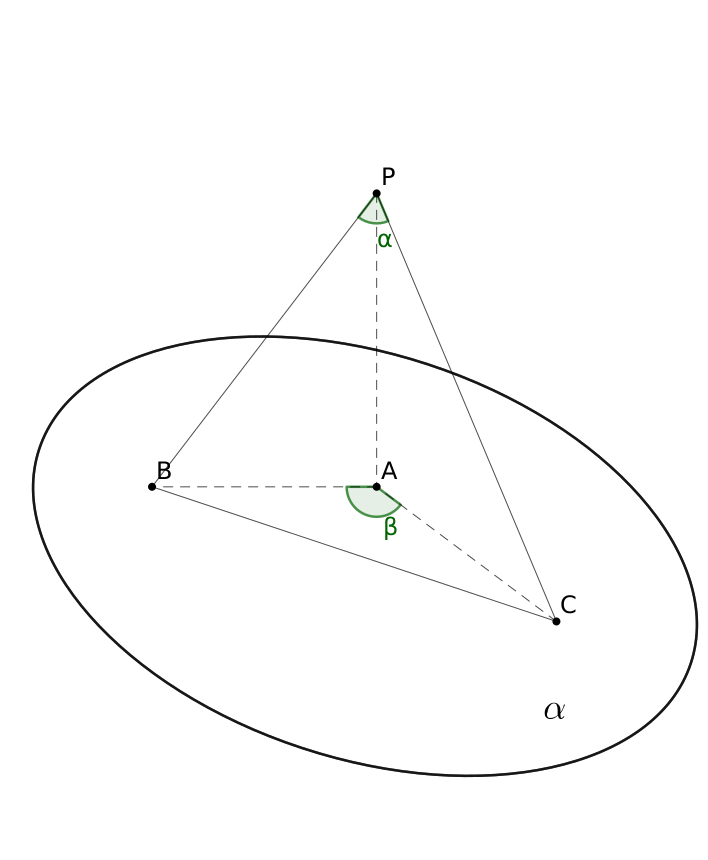
\includegraphics[width=1\textwidth]{{/home/galqiwi/geoma/7.11}.png}
\end{figure}


\end{document}